
%%%%%%%%%%%%%%%%%%%%%%%%%%%%%%%%%%%%%%%%%%%%%%%%%%%%%%%%%%%%%%%%%%%%%%%%%%%%%%%%
%
% Results
%
%%%%%%%%%%%%%%%%%%%%%%%%%%%%%%%%%%%%%%%%%%%%%%%%%%%%%%%%%%%%%%%%%%%%%%%%%%%%%%%%

\section{Results}
\label{sec:results}

%%%%%%%%%%%%%%%%%%%%%%%%%%%%%%%%%%%%%%%%%%%%%%%%%%%%%%%%%%%%%%%%%%%%%%%%%%%%%%%%


With our catalog of matched dark matter halos, we are able to directly compare differences in halo properties arising from initialization with \lpt\ vs \za.  We consider halos on a pair--by--pair basis as well as the entire sample as a whole.  Overall, we find \lpt\ halos to have undergone more growth at a given redshift than their \za\ counterparts.




%~~~~~~~~~~~~~~~~~~~~~~~~~~~~~~~~~~~~~~~~~~~~~~~~~~~~~~~~~~~~~~~~~~~~~~~~~~~~~~~
\subsection{Individual halo pairs}
%~~~~~~~~~~~~~~~~~~~~~~~~~~~~~~~~~~~~~~~~~~~~~~~~~~~~~~~~~~~~~~~~~~~~~~~~~~~~~~~


We compare morphologies, density profiles, and various other halo properties for halo pairs on an individual halo--by--halo basis by eye for several of the most massive halos.  Morphologies appear fairly similar for most halos, indicating good halo matches between simulations.  However, some pairs display a differences in central morphology, in which one halo will have more than one density peak, or in the case of both halos having multiple density peaks, one halo having a larger separation between peaks than the other.  We interpret these cases to be examples of differences in merger epochs, in which case one halo may still be undergoing a major merger, while it's companion is in a more relaxed post-merger state.  We give an example of one such pair at $z = 6$ in Figure~\ref{fig:halo-pair}.  The top two rows show density projections of the central nuclear region for a large \lpt\ and matching \za\ halo (first and second rows, respectively).  We find  the \za\ halo to contain two distinct density peaks with a separation of $\sim 10$ kpc, while the \lpt\ halo displays only a single core.  On the third and fourth rows, we plot the density profiles of the same two halos (\lpt\ and \za, respectively).  Here, with nearly identical virial radii, it is readily seen that the smaller $R_{\mathrm{s}}$ for the \lpt\ halo produces a larger concentration value than is derived for the \za\ halo.




%~~~~~~~~~~~~~~~~~~~~~~~~~~~~~~~~~~~~~~~~~~~~~~~~~~~~~~~~~~~~~~~~~~~~~~~~~~~~~~~
\subsection{Difference distributions of halo properties}
%~~~~~~~~~~~~~~~~~~~~~~~~~~~~~~~~~~~~~~~~~~~~~~~~~~~~~~~~~~~~~~~~~~~~~~~~~~~~~~~


\begin{figure*}[t]
	\centering
	\begin{subfigure}{}
		\includegraphics[width=0.48\linewidth]{diff-hist_Mvir_snap040_(0.0-1.0).eps}
	\end{subfigure}
	~
	\begin{subfigure}{}
		\includegraphics[width=0.48\linewidth]{diff-hist_c_snap040_(0.0-1.0).eps}
	\end{subfigure}
	\\
	\begin{subfigure}{}
		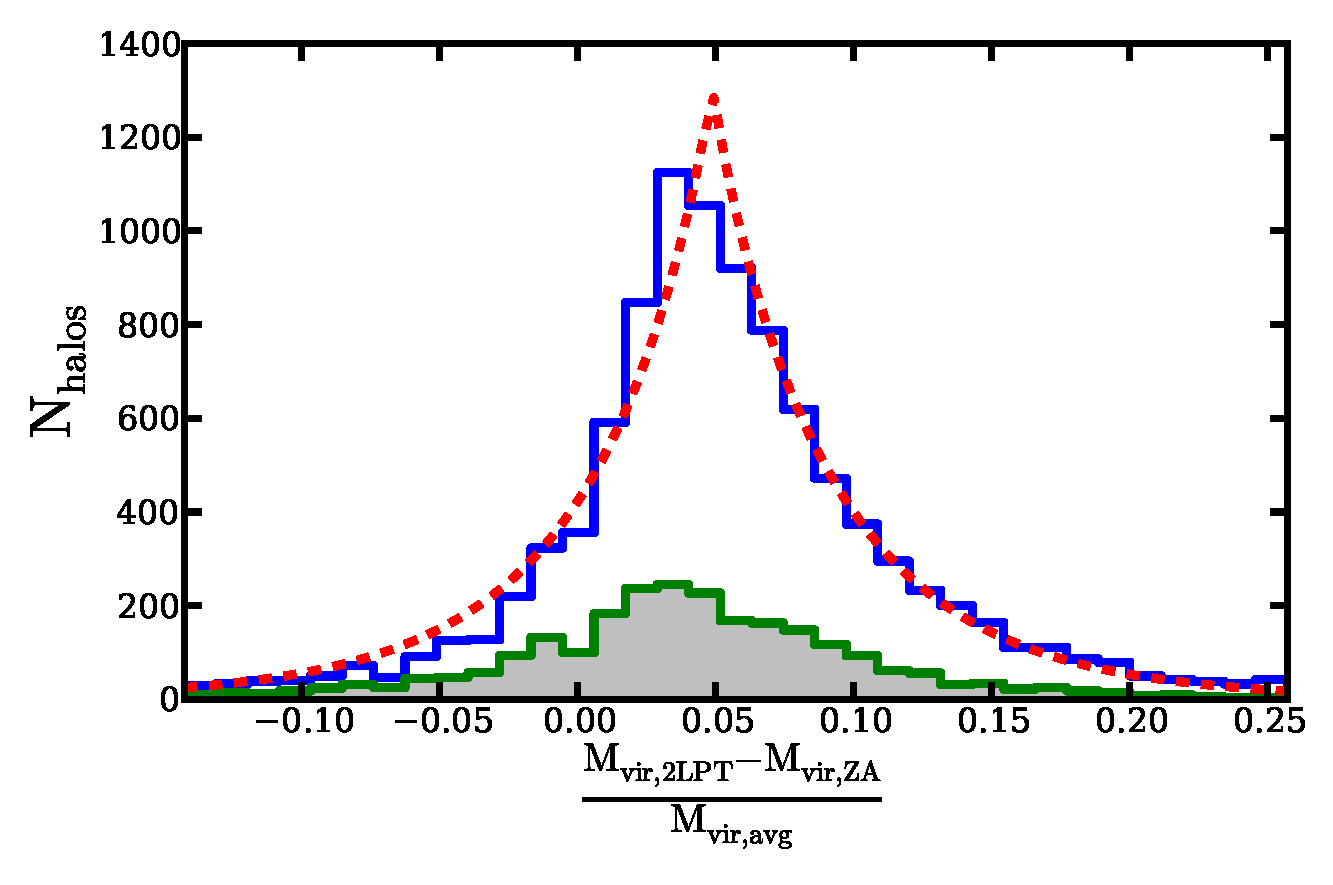
\includegraphics[width=0.48\linewidth]{diff-hist_Mvir_snap050_(0.0-1.0).eps}
	\end{subfigure}
	~
	\begin{subfigure}{}
		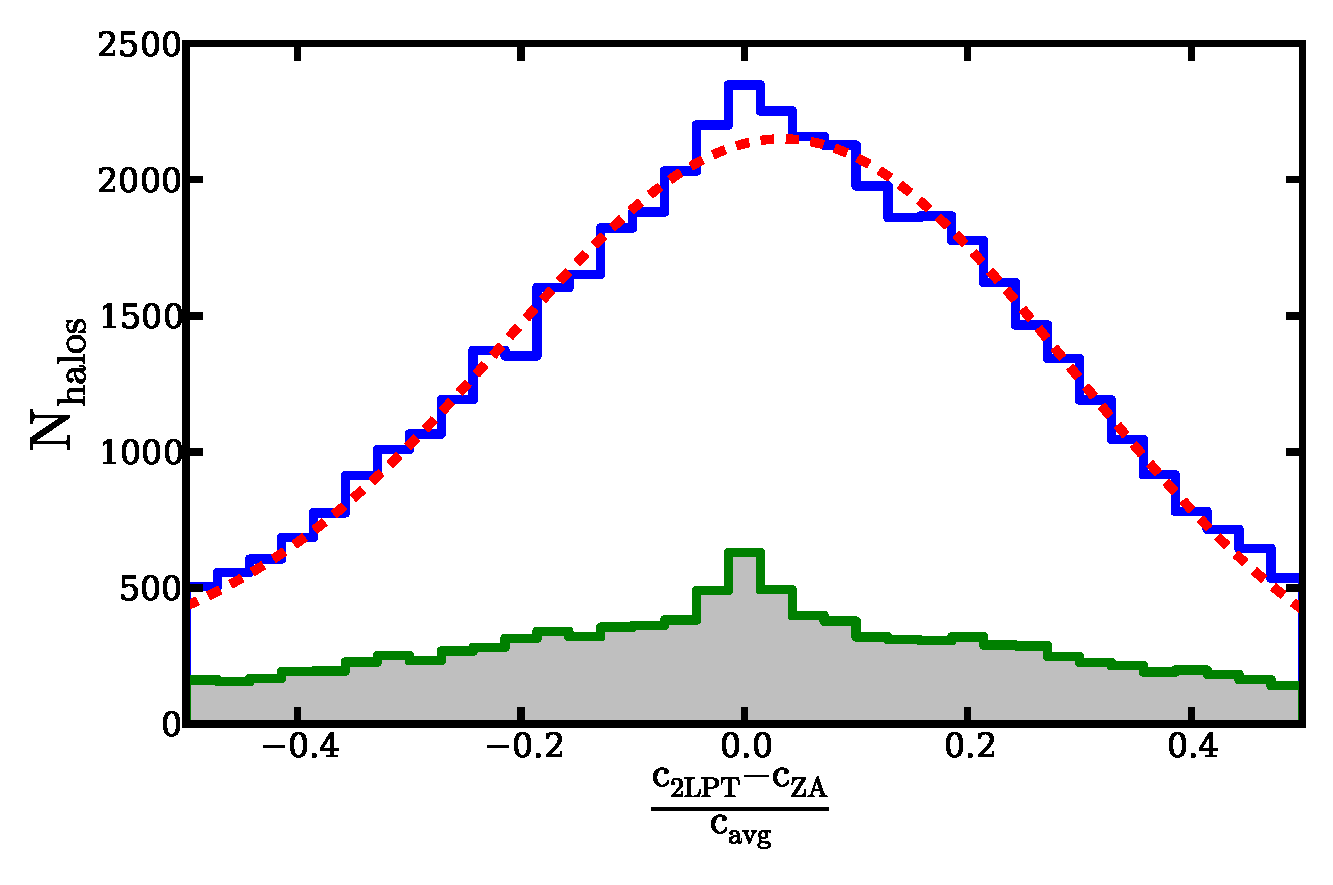
\includegraphics[width=0.48\linewidth]{diff-hist_c_snap050_(0.0-1.0).eps}
	\end{subfigure}
	\\
	\begin{subfigure}{}
		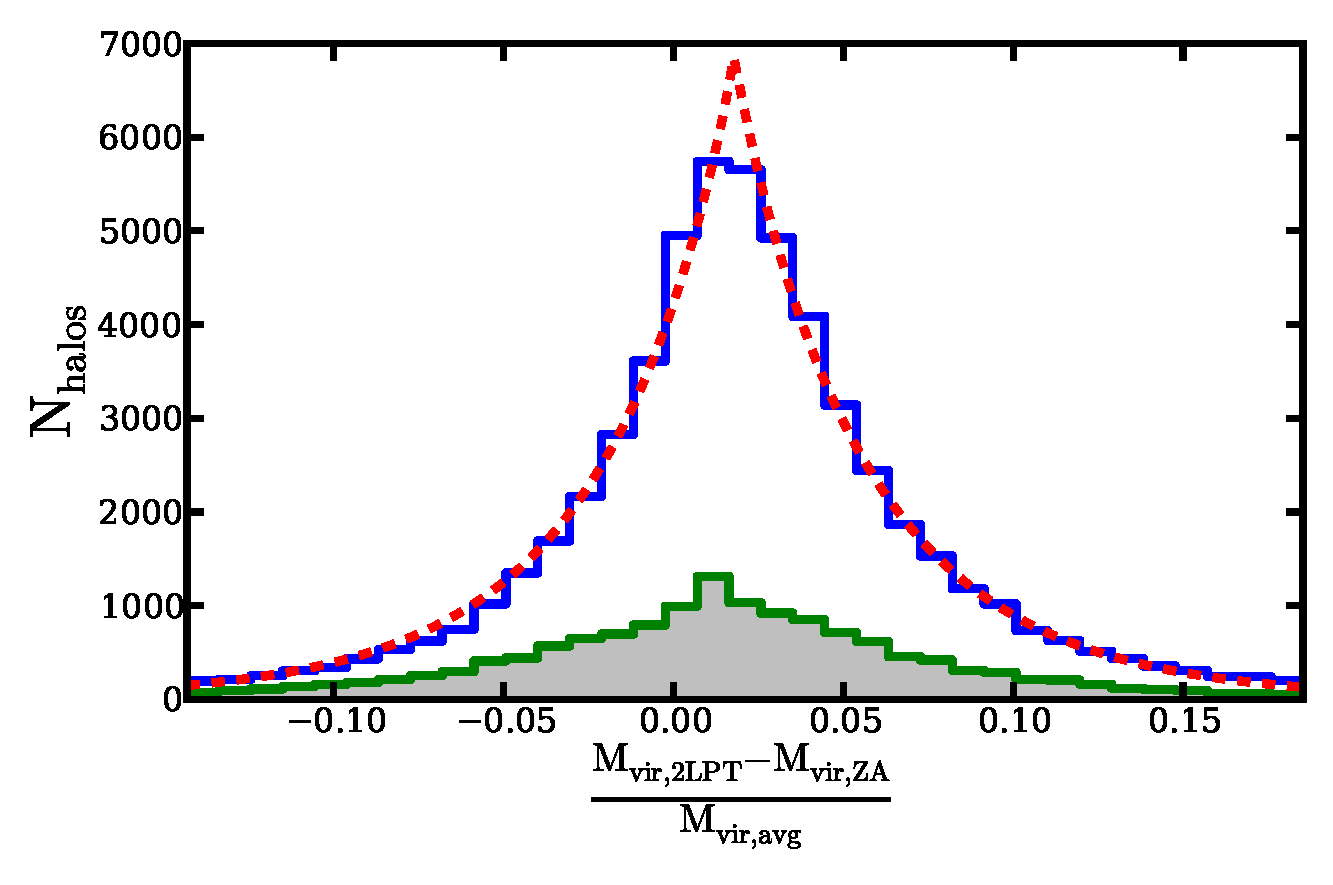
\includegraphics[width=0.48\linewidth]{diff-hist_Mvir_snap061_(0.0-1.0).eps}
	\end{subfigure}
	~
	\begin{subfigure}{}
		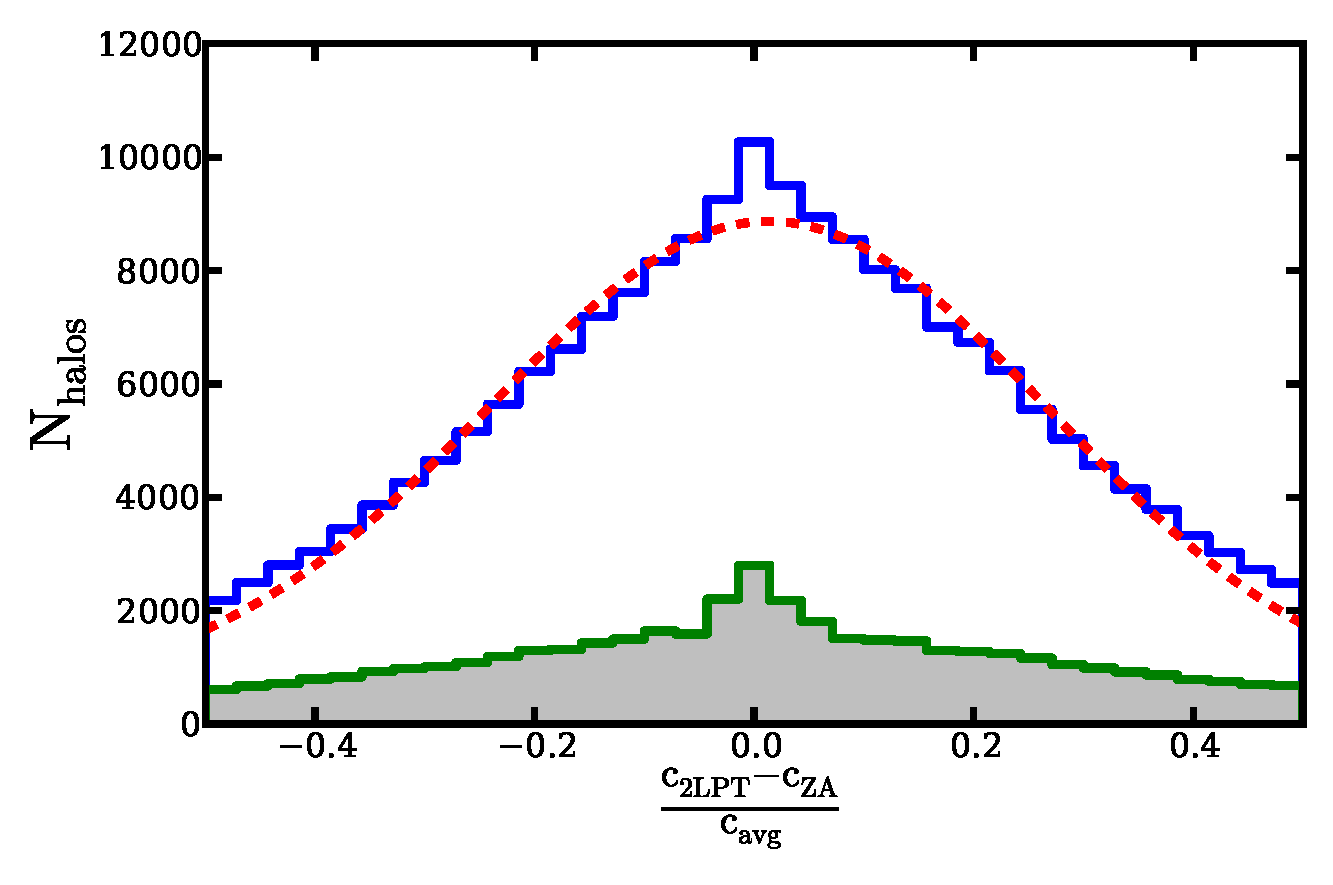
\includegraphics[width=0.48\linewidth]{diff-hist_c_snap061_(0.0-1.0).eps}
	\end{subfigure}
	\caption[Histograms of $\Delta M_{\mathrm{vir}}$ and $\Delta c$]{\footnotesize Histograms of $\Delta M_{\mathrm{vir}}$ (\textit{left column}) and $\Delta c$ (\textit{right column}) for snapshots at $z = 14.7$, $z = 10.3$, and $z = 6.0$ (\textit{top, middle, and bottom panels, respectively}).  The small gray-filled histograms count only the top 25\% most massive halos.  The main histograms are fit with a generalized normal distribution with parameters for mean, scale, and shape, overplotted as the red dashed line.  The shape parameter allows a variable excess kurtosis and the additional inclusion of distribution shapes other than Gaussian.  The distribution for $\Delta M_{\mathrm{vir}}$ has a positive mean and heavier \lpt\ halos, with the most pronounced difference at high redshift.  The skew of the distribution is also the most positive at high redshift, and shifts toward symmetry by $z = 6$.  The $\Delta c$ distribution remains symmetric about zero, with a mean of zero and negligible skew.  Both distributions have excess kurtosis consistently larger than that of a standard Gaussian distribution, with a sharp peak and heavy tails.}
	\label{fig:diff-hist_Mvir}
\end{figure*}

Expanding to an analysis of the halo population as a whole, we consider distributions of halo virial mass $M_{\mathrm{vir}}$, concentration $c$, central density offset $X_{\mathrm{off}}$, defined as the distance between the halo density peak and the halo center of mass \citep{2013ApJ...762..109B}, and a number of other halo parameters.  For each quantity $q$, we create histograms of $\Delta q$, the normalized difference in $q$ between halos in the \lpt\ and \za\ simulations
\begin{equation} \label{eq:delta_q}
	\Delta q = \frac{q_{\lpt} - q_{\za}}{q_{\mathrm{avg}}}
\end{equation}
for each simulation snapshot.  Of these, distributions for $\Delta M_{\mathrm{vir}}$ and $\Delta c$ are the most interesting, with the remainder mostly conforming to the pattern of Gaussians centered about $\Delta q = 0$.

We briefly note, however, that the symmetry of distributions for relaxation-tracking parameters like $\Delta X_{\mathrm{off}}$ might be unexpected at first glance.  As noted above, \lpt\ halos should have more rapid evolution and potentially earlier mergers than their \za\ counterparts, suggesting that we would preferentially find them in a more relaxed state.  However, the lack of average difference between \lpt\ and \za\ indicates that the picture is not as simple as this.  Nuclear displacement may be caught, for example, at a larger value after periapsis passage, while a less-evolved merger may be caught closer to periapsis and thus appear with smaller $X_{\mathrm{off}}$.

We plot histograms of $\Delta M_{\mathrm{vir}}$ and $\Delta c$ in the left and right columns, respectively, of Figure~\ref{fig:diff-hist_Mvir} for three representative timesteps at redshifts of $z = 14.7$, $z = 10.3$, and $z = 6.0$.  For each panel, the blue histogram includes the entire included halo sample, and the smaller gray-filled green histogram includes only the top 25\% most massive halos.  Fits to the primary histograms are overplotted as red dashed curves.

We note that much of our data appears centrally peaked and not well described by a standard Gaussian distribution.  Therefore, for each distribution, in order to additionally account for excess kurtosis, we fit a generalized normal distribution \citep{doi:10.1080/02664760500079464} with probability density function
\begin{equation} \label{eq:generalized_normal}
	f(x) = \frac{ \beta }{2 \alpha \Gamma(1 / \beta)} e^{\left( \left| x - \mu \right| / \alpha \right)^{\beta}},
\end{equation}
where $\mu$ is the mean, $\alpha$ is the scale parameter, $\beta$ is the shape parameter, and $\Gamma$ is the gamma function
\begin{equation} \label{eq:gamma_function}
	\Gamma(t) = \int_{0}^{\infty} x^{t-1} e^{-x} \dd x.
\end{equation}
The shape parameter $\beta$ is restricted to $\beta \geq 1$.  This allows the distribution to potentially vary from a Laplace distribution ($\beta = 1$) to a uniform distribution ($\beta = \infty$) and includes the normal distribution ($\beta = 2$).  The distribution has variance
\begin{equation} \label{eq:variance}
	\sigma^{2} = \frac{ \alpha^{2} \Gamma(3/\beta) }{ \Gamma(1/\beta) }
\end{equation}
and excess kurtosis
\begin{equation} \label{eq:kurtosis}
	\gamma_{2} = \frac{ \Gamma(5/\beta) \Gamma(1/\beta) }{ \Gamma(3/\beta)^{2} } - 3.
\end{equation}
The distribution is symmetric, and thus has no skewness by definition.  As such, the values for skew presented below are measured directly from the data and do not rely on the fit to the histograms.

From a high redshift, we find a tendency for \lpt\ halos to be more massive.  The mean is consistently positive (heavier \lpt\ halos) and is most displaced from zero at high redshift.  The peak of the distribution gradually moves closer to zero as we progress in redshift.  We find the least difference between paired halos for the final snapshot at $z = 6$.  These trends with redshift are discussed in more detail below.

The higher-order moments of the $\Delta M_{\mathrm{vir}}$ distribution are of interest as well, as we find significant deviation from the standard Gaussian distribution that one might expect.  We find the distribution to be much closer to a Laplace distribution, with shape parameter consistently sitting at or very close to $\beta = 1$.  When compared to a Gaussian distribution, the larger excess kurtosis implies a sharper central peak and heavier outlier tails.  We note that, as we have required $\beta \geq 1$ when fitting the data in order to not allow the fitting distribution to be more peaked than the Laplace distribution, the kurtosis of the data itself could potentially be even higher than what is represented by the fit.

As we use the symmetrical generalized normal distribution as our fit function, the skewness of the data is unable to be measured from the fit itself.  However, a qualitative deviation from symmetry can be readily observed.  By $z = 6$, we end up with a rather symmetrical distribution, with both sides of the histogram equally well described by our fit.  However, at higher redshift, we note a marked increase in skewness and deviation from this symmetry.  As redshift increases, we observe an increasing difference between the fit curve and the bins to the left of the histogram peak.

We find no no overall preference for more concentrated \lpt\ or \za\ halos.  In contrast to the $\Delta M_{\mathrm{vir}}$ histograms , $\Delta c$ shows very little deviation from symmetry about zero.  Throughout the simulation, we find the distributions to have a mean close to zero and negligible skew.  The widths of the distributions are much wider than those for $\Delta M_{\mathrm{vir}}$.  As with mass, concentration histograms are sharply peaked with heavy tails.




%~~~~~~~~~~~~~~~~~~~~~~~~~~~~~~~~~~~~~~~~~~~~~~~~~~~~~~~~~~~~~~~~~~~~~~~~~~~~~~~
\subsection{Trends with redshift}
%~~~~~~~~~~~~~~~~~~~~~~~~~~~~~~~~~~~~~~~~~~~~~~~~~~~~~~~~~~~~~~~~~~~~~~~~~~~~~~~


\begin{figure*}[t]
	\centering
	\begin{subfigure}{}
		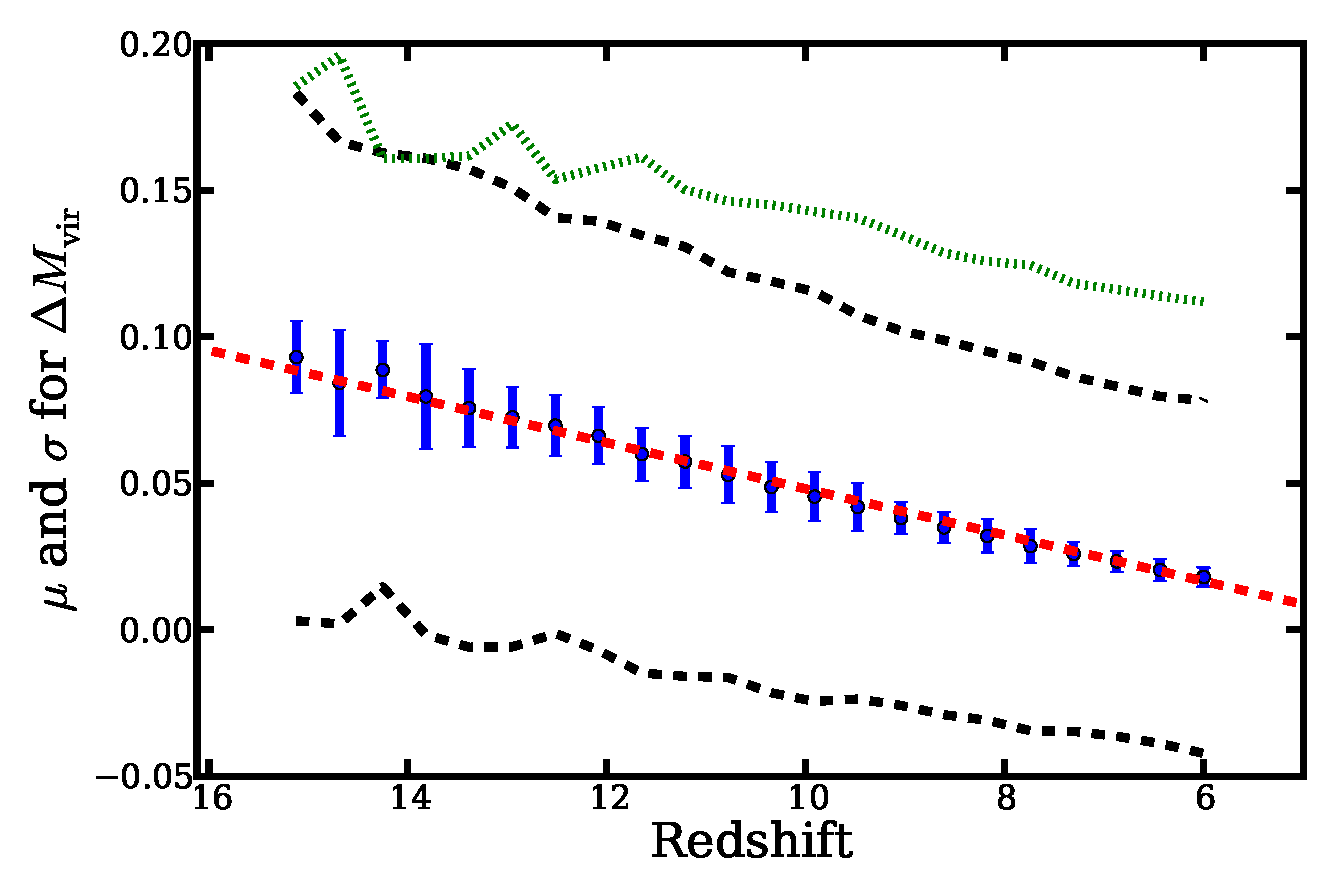
\includegraphics[width=0.48\linewidth]{mean_stdev_Mvir.eps}
	\end{subfigure}
	~
	\begin{subfigure}{}
		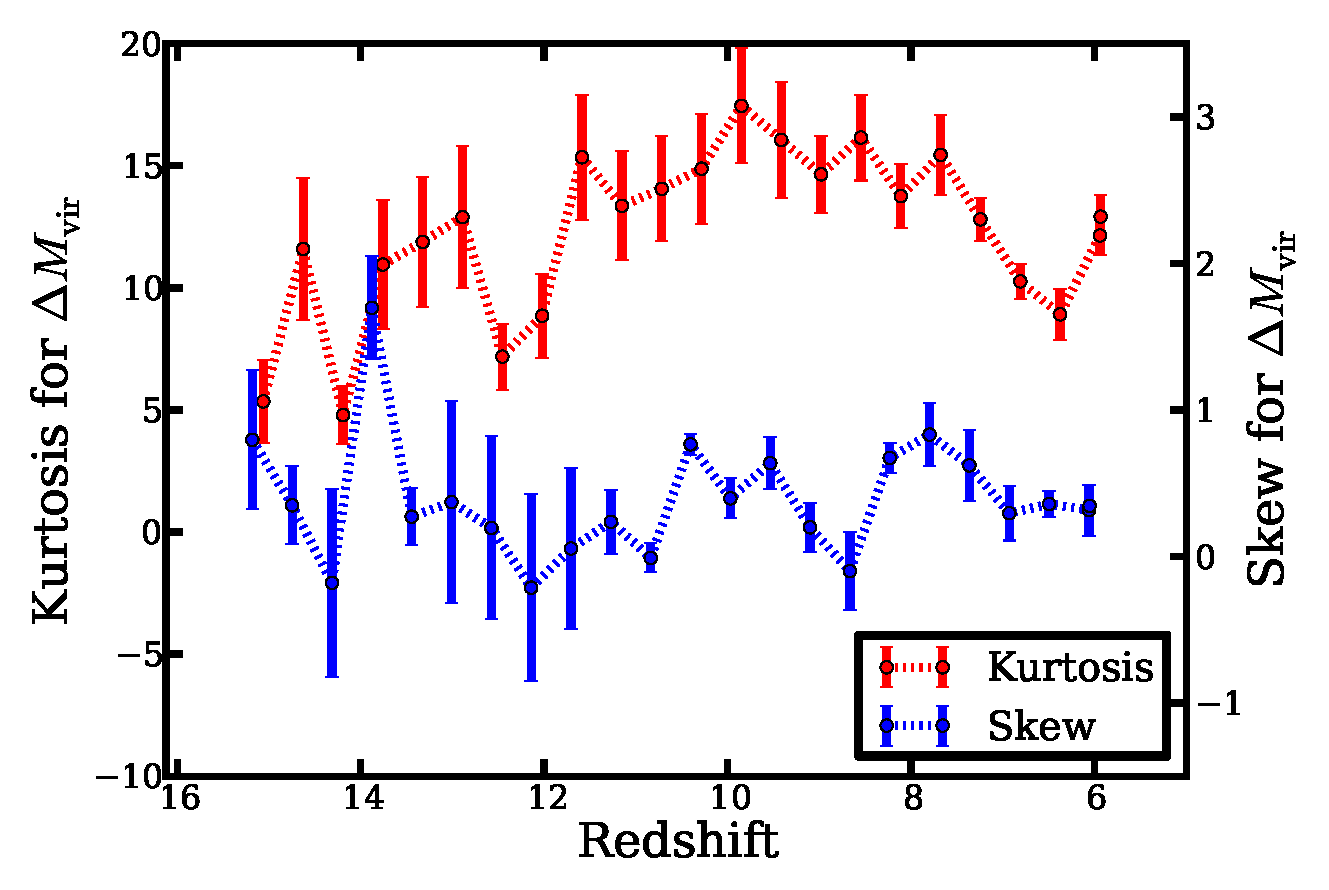
\includegraphics[width=0.48\linewidth]{skew_kurtosis_Mvir.eps}
	\end{subfigure}
	\\
	\begin{subfigure}{}
		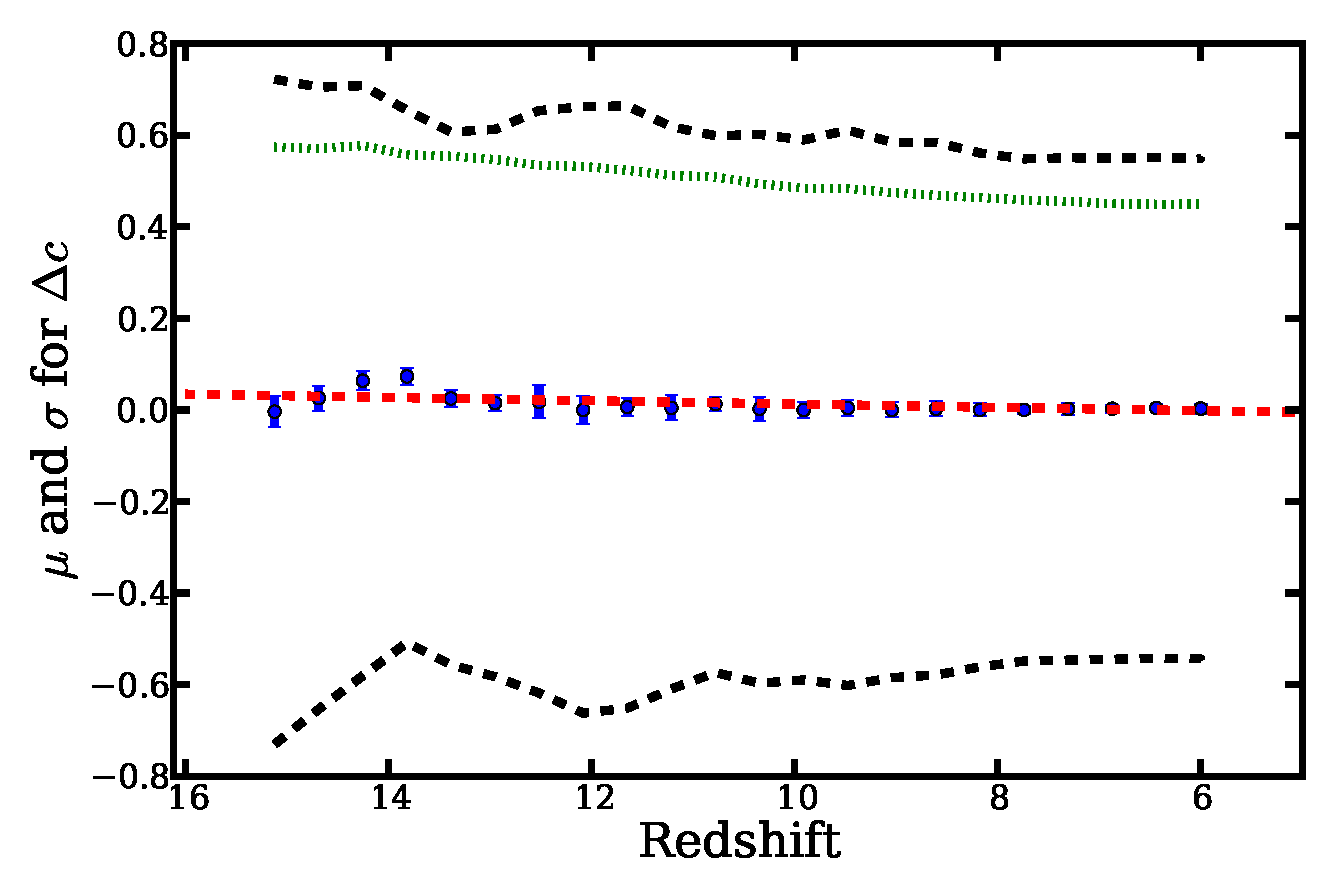
\includegraphics[width=0.48\linewidth]{mean_stdev_c_rockstar.eps}
	\end{subfigure}
	~
	\begin{subfigure}{}
		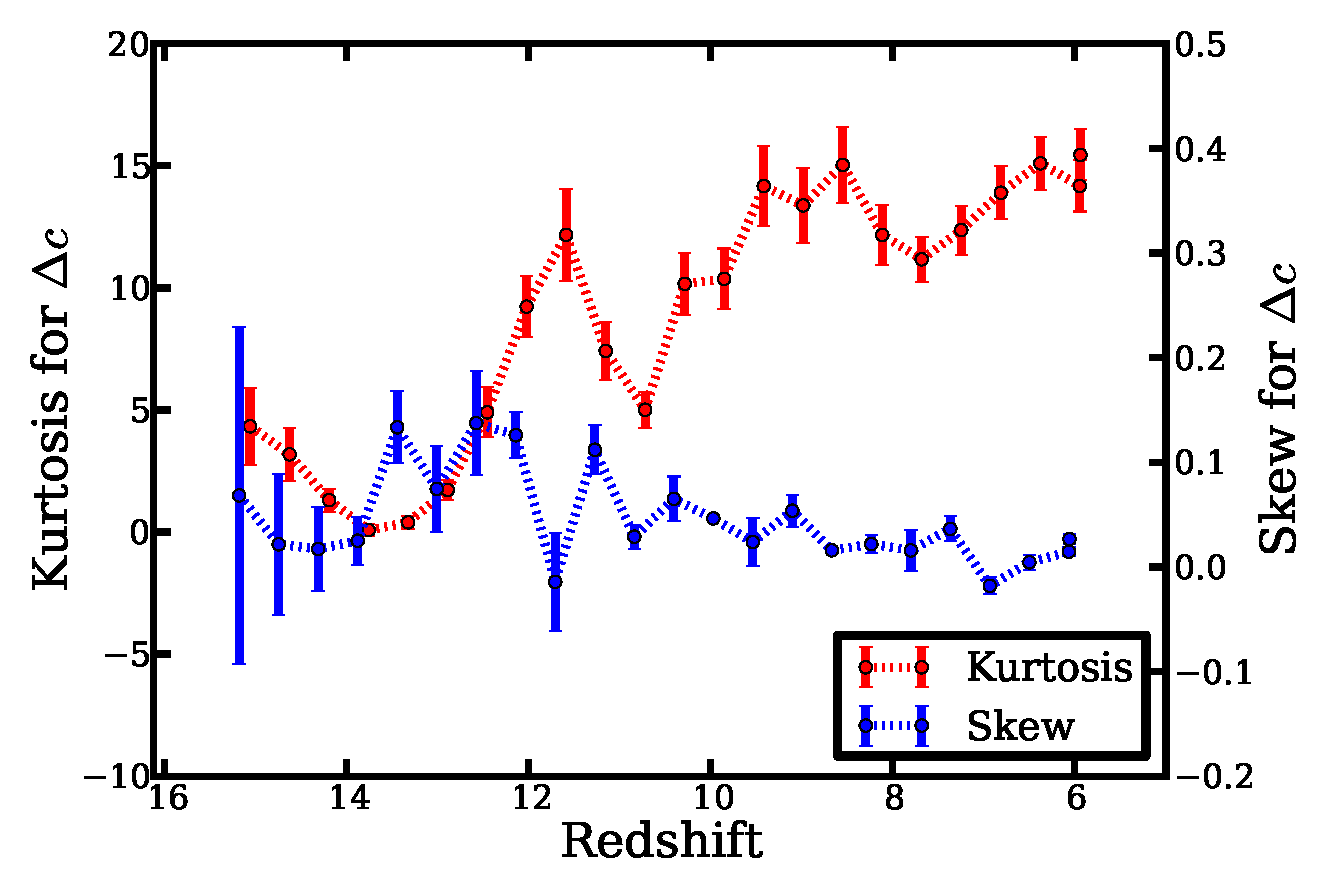
\includegraphics[width=0.48\linewidth]{skew_kurtosis_c_rockstar.eps}
	\end{subfigure}
	\caption[Statistics as functions of redshift for generalized normal fits]{\footnotesize Mean, standard deviation, and RMS (\textit{left column}) and skew and excess kurtosis (\textit{right column}) as functions of redshift for $\Delta M_{\mathrm{vir}}$ (\textit{top row}) and $\Delta c$ (\textit{bottom row}).  In the left column, $\mu$ is plotted as blue points, and $\mu \pm \sigma$ is plotted as the black dashed line, and RMS values are plotted as a green dotted line.  The red dashed line is a linear fit to the mean.  We find a significant trend for $\mu$ for $\Delta M_{\mathrm{vir}}$ to be more positive at higher redshift and gradually shift toward zero as the simulation progresses.  The mean for $\Delta c$, however, remains at or very near zero for most of the simulation.  The $\Delta M_{\mathrm{vir}}$ and $\Delta c$ distributions narrow over time, with a slight decrease in $\sigma$.  In the right column, we plot skew (blue line) and excess kurtosis (red line).  Skew is positive for much of the simulation for $\Delta M_{\mathrm{vir}}$, but is much smaller for $\Delta c$.  Kurtosis is large (much more peaked than Gaussian) for both $\Delta M_{\mathrm{vir}}$ and $\Delta c$ throughout much of the simulation, and especially at later redshift.}
	\label{fig:fit_trends}
\end{figure*}

In Figure~\ref{fig:fit_trends}, we more quantitatively assess the time progression of our various trends hinted at in Figure~\ref{fig:diff-hist_Mvir}.  Here, we plot the mean, root mean square (RMS), standard deviation, skew, and kurtosis for $\Delta M_{\mathrm{vir}}$ and $\Delta c$ as functions of redshift.  Uncertainty in the mean is estimated directly by the least squares fitting routine.

As our fitting distributions are symmetrical and skew must therefore be measured directly from the data, in order to derive uncertainties for skew, we measure the skew of the distributions for each of our three simulation boxes individually as well as for the single stacked data set.  Uncertainty in skew is then simply the standard deviation of the mean of the skew of the three individual boxes.

Determining the uncertainty in the kurtosis is slightly more involved, as kurtosis is determined by a transformation of the generalized normal distribution's shape parameter $\beta$ according to (\ref{eq:kurtosis}).  Following the standard procedure for propagation of uncertainty, we calculate the standard deviation of the kurtosis as
\begin{align} \label{eq:kurt_err_partial}
    s_{\gamma_{2}} &= \sqrt{ \left( \frac{\diff \gamma_{2}}{\diff \beta} \right)^{2} s_{\beta}^{2} } \\
        &= s_{\beta} \frac{\diff}{\diff \beta} \left[ \frac{\Gamma(5/\beta) \Gamma(1/\beta)}{\Gamma(3/\beta)^{2}} - 3 \right].
\end{align}
The derivative of the gamma function is
\begin{equation} \label{eq:gamma_prime}
    \Gamma'(x) = \Gamma(x) \psi_{0}(x)
\end{equation}
where the digamma function $\digamma$ is the derivative of the logarithm of the gamma function and is given by
\begin{equation} \label{eq:digamma}
    \digamma(x) = \int_{0}^{\infty} \left( \frac{e^{-t}}{t} - \frac{e^{-xt}}{1 - e^{-t}} \right) \dd t
\end{equation}
if the real part of $x$ is positive.  Now, taking the derivative of $\gamma_{2}$ and doing a bit of algebra gives us
\begin{equation} \label{eq:kurt_err}
    s_{\gamma_{2}} = s_{\beta} \frac{1}{\beta^{2}} \left( \gamma_{2} + 3 \right) \left[ 6 \digamma(3/\beta) - 5 \digamma(5/\beta) - \digamma(1/\beta) \right],
\end{equation}
with which we can find the uncertainty in the kurtosis given the value and uncertainty of the shape parameter $\beta$ estimated from the least squares fit routine.

The mean for $\Delta M_{\mathrm{vir}}$ is positive and highest at high redshift, trending toward zero by the end of the simulation.  Distributions for $\Delta c$ retain means close to and consistent with zero.  Standard deviation decreases slightly for both $\Delta M_{\mathrm{vir}}$ and $\Delta c$.

\begin{table}[t]
	\centering
	\caption{Coefficients for linear least squares fits from Figure~\ref{fig:fit_trends}.}
	\begin{tabular}{ l  r  r }
		\toprule
		& \multicolumn{1}{c}{$\Delta M_{\mathrm{vir}}$} & \multicolumn{1}{c}{$\Delta c$} \\
		\cmidrule(l){2-3}
		A &  $(7.88 \pm 0.17) \times 10^{-3}$ &  $(3.62 \pm 0.95) \times 10^{-3}$ \\
		B & $(-3.07 \pm 0.14) \times 10^{-2}$ & $(-2.34 \pm 0.84) \times 10^{-2}$ \\
		\bottomrule
	\end{tabular}
	\label{tab:coeffs}
\end{table}

We find least square linear fits for both mean $\Delta M_{\mathrm{vir}}$ vs $z$ and mean $\Delta c$ vs $z$.  Coefficients for slope $A$ and y-intercept $B$ for the fit equation $\mu = A z + B$ are given in Table~\ref{tab:coeffs} for both cases.  (Note the reversed redshift axes for the sign of the slopes.)  We find a significant trend for $\Delta M_{\mathrm{vir}}$, with a slope $\sim 46 \sigma$ from zero.  Conversely, the slope for $\Delta c$ is much smaller and, considering the larger spread of the underlying distributions, can be considered negligible.  For $\Delta M_{\mathrm{vir}}$, the y-intercept coefficient $B$ likely has little meaning in terms of the actual behaviour at $z = 0$, as we expect the trend to level out at later redshift.

We do note, however, that the mean can be deceiving as an indicator of total difference between halo populations, especially when it is close to zero as with concentration.  It should be noted that while the mean can indicate a lack of average difference between the whole sample of \lpt\ and \za\ halos, there can still be very large discrepancies between many individually paired halos.  We visualize this by plotting the RMS of $\Delta M_{\mathrm{vir}}$ and $\Delta c$, which is plotted as a green dotted line.  Unlike the mean, standard deviation,and kurtosis, which are measured from fits to the histograms, RMS is measured directly from the data and is not dependent on fitting.  The large RMS values are indicative of how much overall difference can arise between \lpt\ and \za\ halos, even though the differences may average to zero when considering the entire population.  The RMS for both $\Delta M_{\mathrm{vir}}$ and $\Delta c$ starts highest at high redshift and steadily decreases throughout the simulation, reaching a minimum by $z = 6$.

Additionally, it is of interest to consider the percentage of halo pairs that are ``wrong'' at some given time, regardless of whether the quantity is higher in \lpt\ or \za.  For example, if we count halos outside a slit of width $\epsilon = \pm 10\%$ around $\Delta q = 0$, we find that by $z = 6$, 14.6\% of halo pairs still have substantially mismatched masses.  Likewise, 74.3\% have mismatched concentrations.  It is evident that many halo pairs can have markedly different growth histories, even when the ensemble halo populations have similar distributions.

Kurtosis is consistently large (more peaked than a Gaussian distribution) for both mass and concentration, with a slight increasing trend throughout the simulation for concentration.  Skew is positive for much of the simulation for mass, but is much smaller for concentration.  These higher moment deviations from Gaussianity hint at the non-linear dynamics at play in halo formation.

The large excess kurtosis indicates a sharper peak and heavier tails than a Gaussian for the underlying distribution.  This may indicate a fair amount of sensitivity to initial differences in halo properties, in that halo pairs that start out within a certain range of the mean are more likely move closer to the mean, while pairs that are initially discrepant will diverge even further in their characteristics.  This is further supported by a kurtosis that increases with time.

The skew at high redshift for $\Delta M_{\mathrm{vir}}$ may give another hint at the non-linear halo formation process.  Runaway halo growth causes more massive halos to favor faster mass accretion and growth.  The positively skewed distributions show a picture of \lpt\ halo growth in which initial differences in mass are amplified the most readily in the earliest forming and most massive halos, again indicating the extra kick-start to halo growth provided by \lpt\ initialization.  While the slight decrease in skew with redshift may be counter-intuitive to this notion, it is likely that rising noise floor of the large amounts of newly formed halos begin to mask the signal from the smaller number of large halos displaying this effect.




%~~~~~~~~~~~~~~~~~~~~~~~~~~~~~~~~~~~~~~~~~~~~~~~~~~~~~~~~~~~~~~~~~~~~~~~~~~~~~~~
\subsection{Trends with halo mass}
%~~~~~~~~~~~~~~~~~~~~~~~~~~~~~~~~~~~~~~~~~~~~~~~~~~~~~~~~~~~~~~~~~~~~~~~~~~~~~~~


\begin{figure*}[t]
	\centering
	\begin{subfigure}{}
		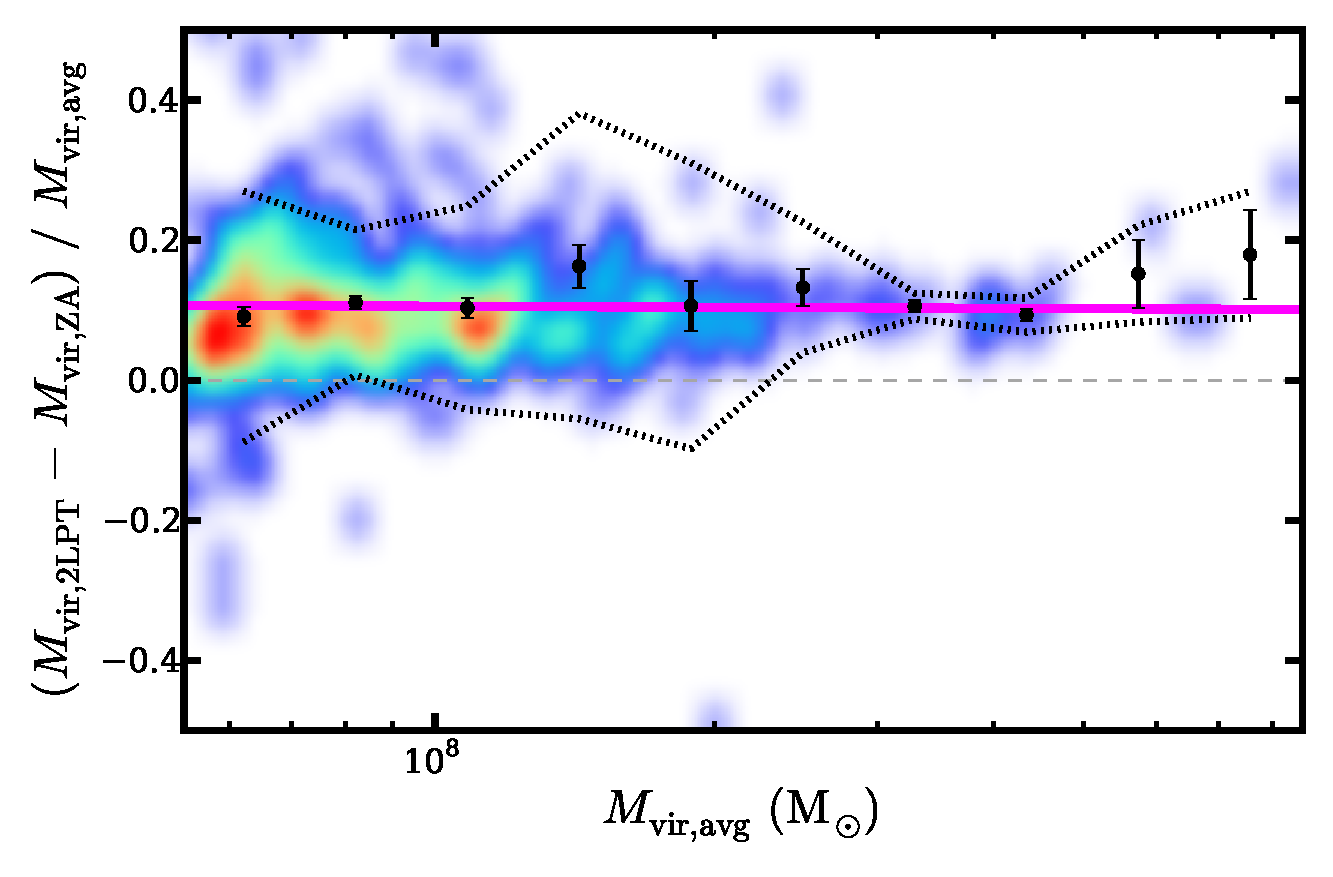
\includegraphics[width=0.48\linewidth]{dM-v-Mavg_snap040.eps}
	\end{subfigure}
	~
	\begin{subfigure}{}
		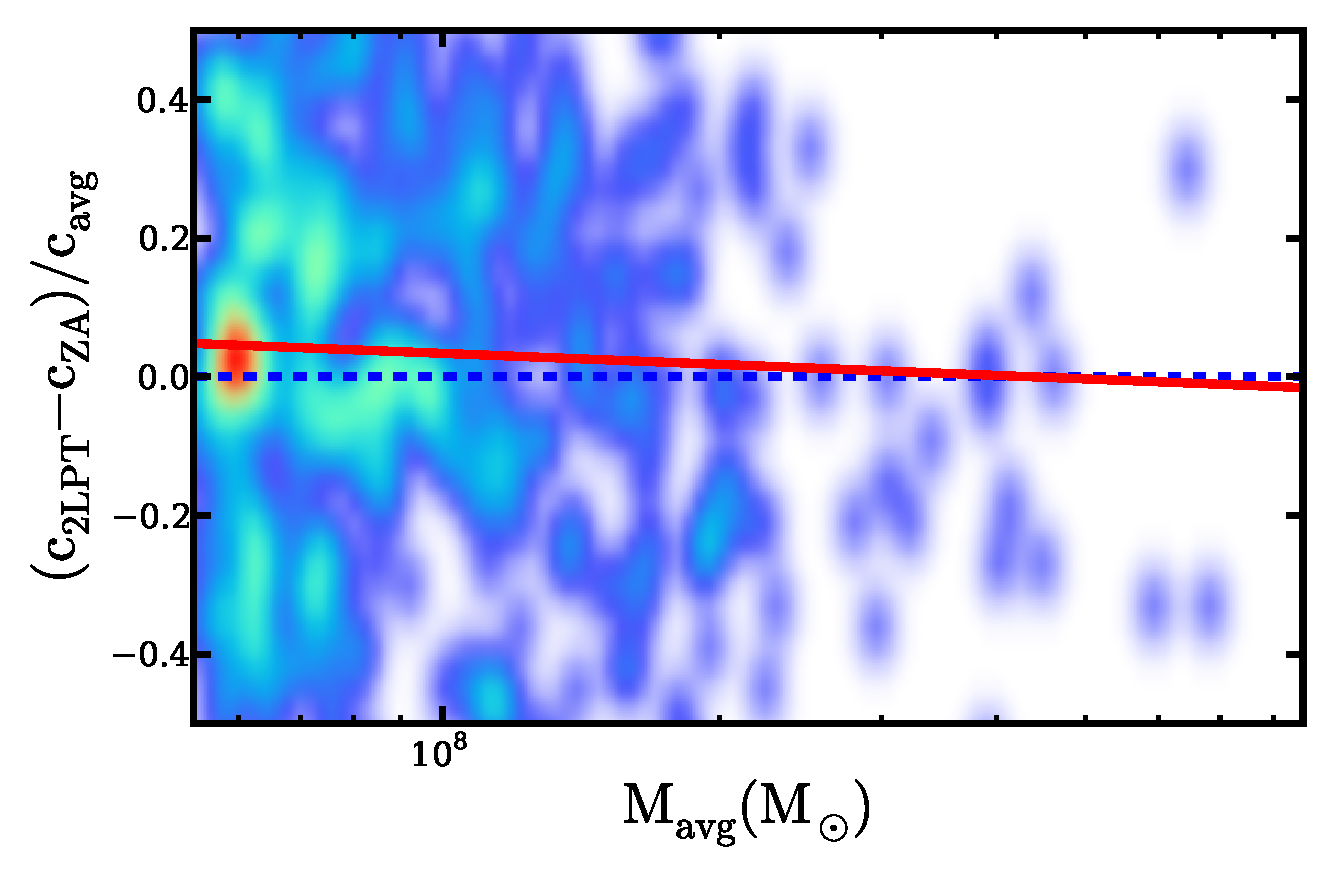
\includegraphics[width=0.48\linewidth]{dc-v-Mavg_snap040.eps}
	\end{subfigure}
	\\
	\begin{subfigure}{}
		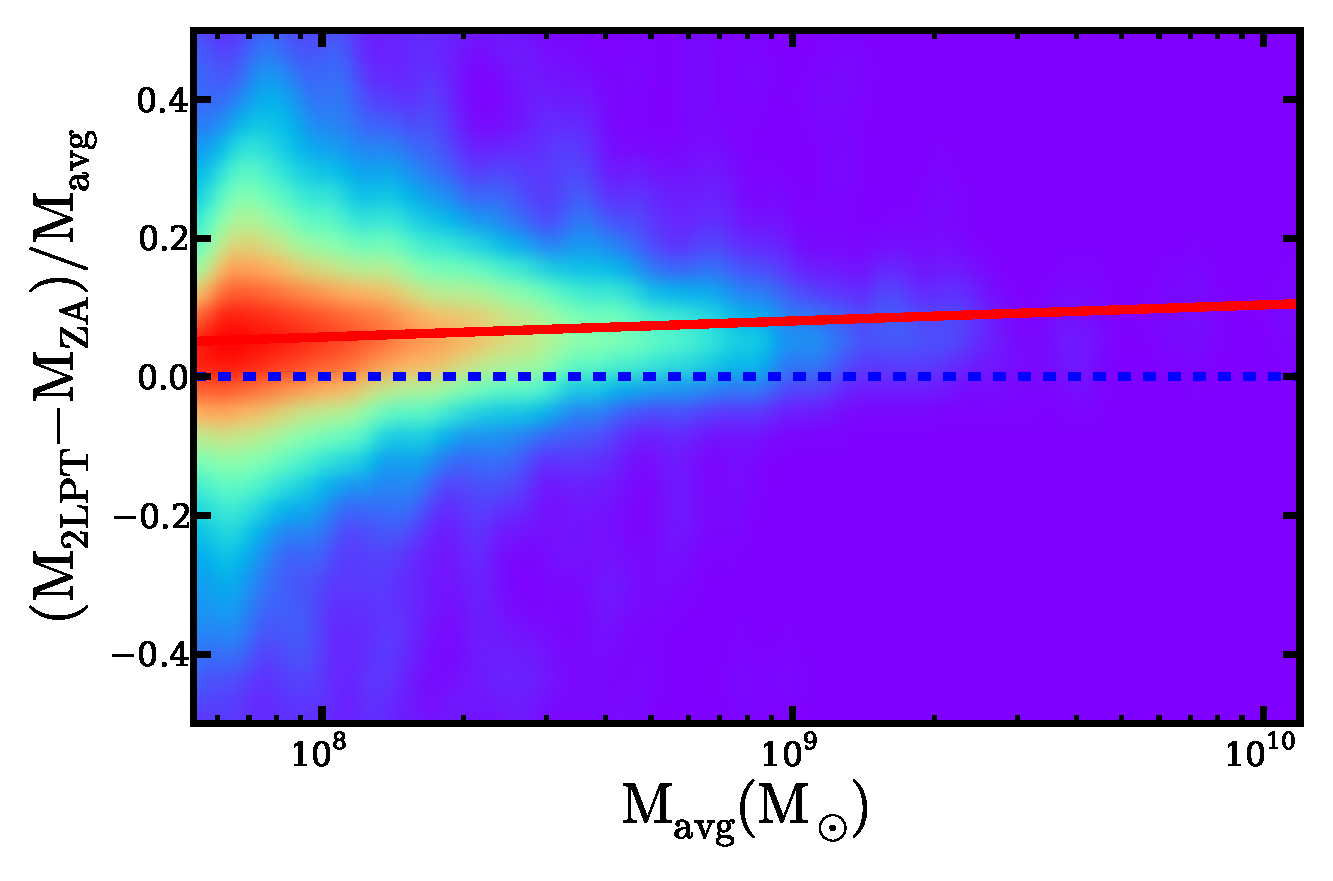
\includegraphics[width=0.48\linewidth]{dM-v-Mavg_snap050.eps}
	\end{subfigure}
	~
	\begin{subfigure}{}
		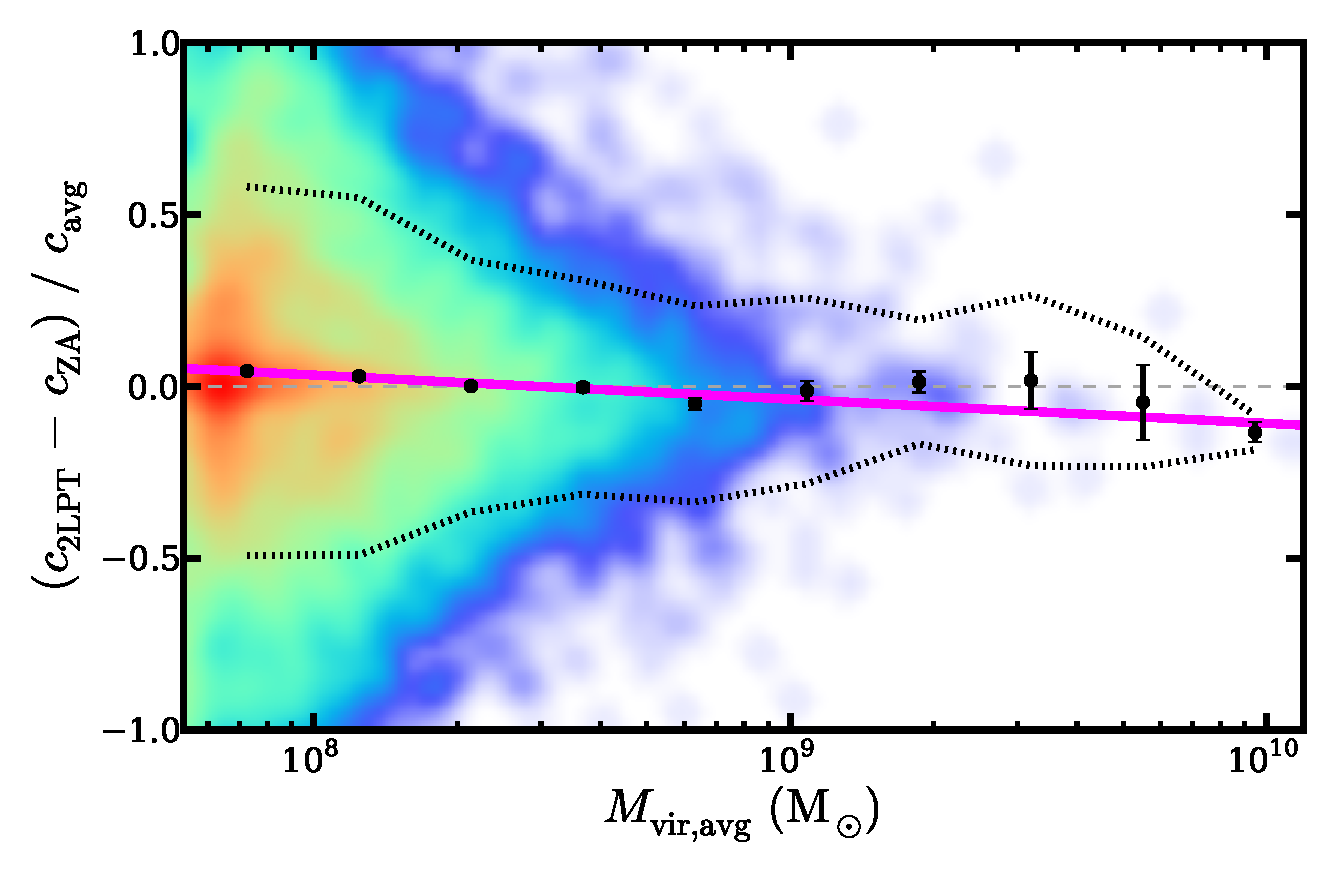
\includegraphics[width=0.48\linewidth]{dc-v-Mavg_snap050.eps}
	\end{subfigure}
	\\
	\begin{subfigure}{}
		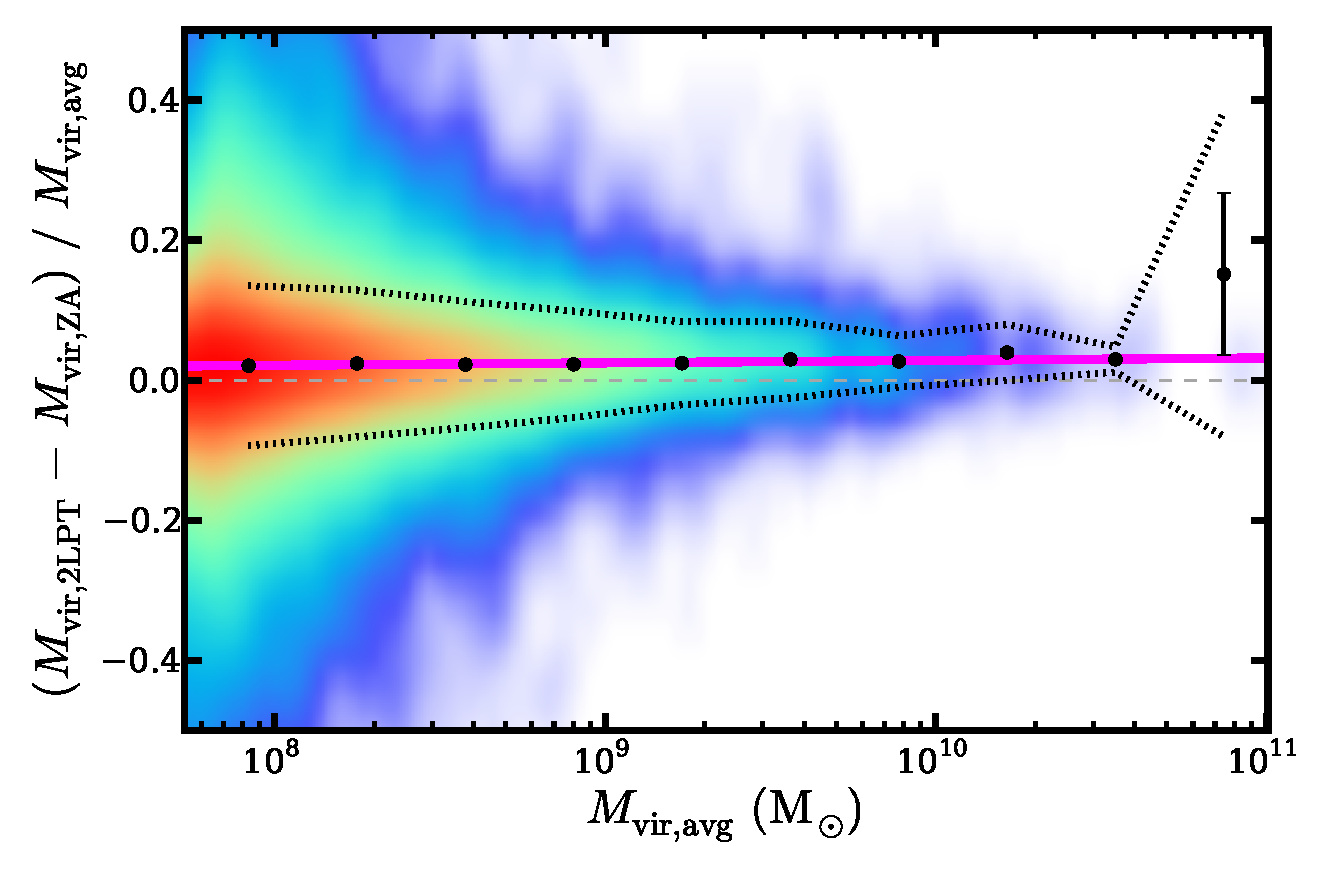
\includegraphics[width=0.48\linewidth]{dM-v-Mavg_snap061.eps}
	\end{subfigure}
	~
	\begin{subfigure}{}
		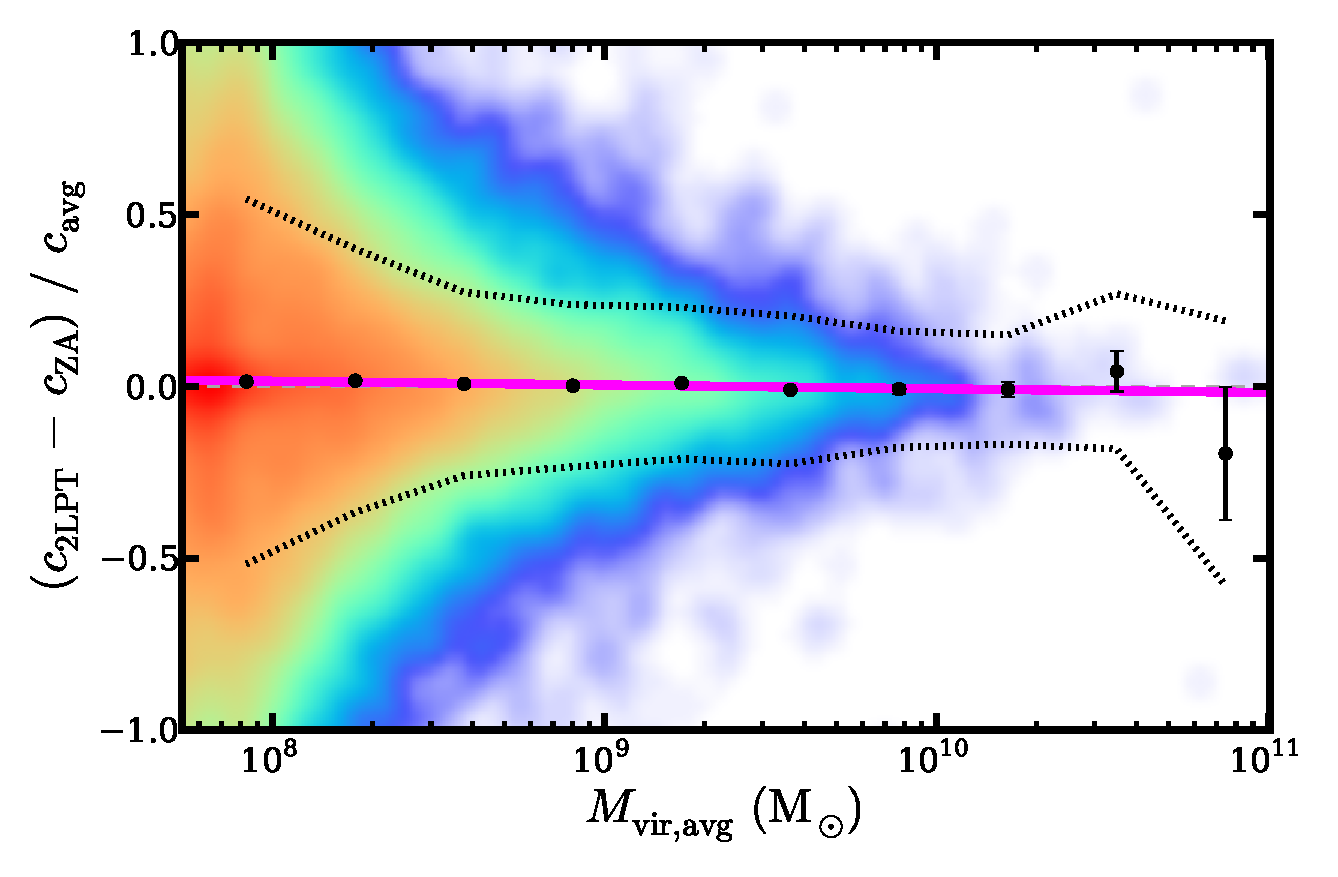
\includegraphics[width=0.48\linewidth]{dc-v-Mavg_snap061.eps}
	\end{subfigure}
	\caption[$\Delta M_{\mathrm{vir}}$ and $\Delta c$ as a function of $M_{\mathrm{vir,avg}}$]{\footnotesize $\Delta M_{\mathrm{vir}}$ (left column) and $\Delta c$ (right column) as functions of $M_{\mathrm{vir,avg}}$.  Halos are counted in 2-D rectangular bins and smoothed with a Gaussian kernel with a logarithmic color scale.  The red line is the least-squares best fit to the data.  The blue dashed line at zero is provided to guide the eye.  The three rows again correspond to snapshots at $z = 14.7$, $z = 10.3$, and $z = 6.0$, respectively.}
	\label{fig:delta-v-Mavg}
\end{figure*}

We consider $\Delta M_{\mathrm{vir}}$ and $\Delta c$ as a function of average halo mass $M_{\mathrm{vir,avg}} = (M_{\mathrm{vir},\lpt} + M_{\mathrm{vir},\za}) / 2$ in Figure~\ref{fig:delta-v-Mavg}.  The data is binned on a 2-D grid with a logarithmic color map for three representative timesteps.  A linear fit to the data is overplotted in red, and a dotted blue line is provided at $\Delta M_{vir} = 0$ and $\Delta c = 0$ to guide the eye.

We find that $\Delta M_{vir}$ tends to increase with increasing $M_{\mathrm{vir,avg}}$, a trend that is, again, most pronounced at high redshift.  \lpt\ halos are consistently more massive than their \za\ counterparts, with the difference increasing with average halo mass.  While less massive halo pairs have a larger spread in the difference in \lpt\ and \za\ mass, more massive halo pairs are more consistently heavier in \lpt\ than in \za.  The slope of the fit line trends towards zero as we progress in redshift, with little average mass dependence by $z = 6$.

We find a small trend for more massive halo pairs to be more concentrated in \za, but this trend is weaker than for $\Delta M_{\mathrm{vir}}$.  This negative slope can be expected, as halo concentartion is expected to decrease with increasing mass \citep{2001MNRAS.321..559B}, and we find high mass halos to be more massive in \lpt\ than in \za.  The data have a larger variance than $\Delta M_{\mathrm{vir}}$, and fits have and overall shallower slope.  Mass dependence all but disappears by $z = 6$.  To reconcile these trends with the symmetrical concentration distributions of Figure~\ref{fig:diff-hist_Mvir}, we note that the trends in mass may be hidden by integration across the entire mass range and still result in overall $\Delta c$ distributions symmetric about zero.




